\documentclass{article}
\usepackage{graphicx}
\usepackage{enumitem}
\usepackage{amsmath}
\usepackage{biblatex}
\usepackage{subcaption}
\usepackage{amssymb}
\usepackage{multicol}
\usepackage{hyperref}

\usepackage[margin=1in]{geometry}

\addbibresource{references.bib}

\graphicspath{{Images/}{./}}

\title{Reinforcement Learning with the Card Game Scoundrel}
\author{Colby Cox}
\date{Due: April 17, 2026}

\begin{document}
\maketitle

\section{Introduction}
Scoundrel is a game whose probability to win is largely influenced by the initial shuffle of the deck. The player can be swarmed by monsters and immediately lose, or swamped by helpful items that can not be used to their fullest. Winning Scoundrel sometimes comes down to a advantageously shuffled spread of items and monsters, but how much is winning within the player's control?

This project originally sought to find a lower bound for the win rate by using reinforcement learning and comparing to a human player. However, after extensive testing, I have determined that the conditions of the game Scoundrel make generalizing it for any set of shuffled cards make learning very difficult. Some other examples of successful implementations of reinforcement learning include Chess and Atari games like Breakout and Pong \cite{mnih_playing_2013}. Chess is highly complex, with an upper bound for the number of legal game states being about $7.7 \times 10^{45}$ \cite{tromp_chess_2026} . Compare this to Scoundrel, which is a deck of 44 cards and thus has 44!, about $2.7 \times 10^{54}$, possible game states at the beginning of the game. Without a highly specific implementation of reinforcement learning capable of generalizing the relationship of the cards for the computer, it makes solving Scoundrel for any deck highly complex. Meanwhile Atari games are much simpler, and have a much smaller number of potential game states than Scoundrel, so their implementation can be much more general. As such, I've reduced the scope to asking if we can find a set of decisions that can beat a given deck without human involvement using reinforecement learning.

\section{The Rules}
Scoundrel was created by Zach Gage and Kurt Bieg, and their rule set can be found at \\ http://www.stfj.net/art/2011/Scoundrel.pdf \cite{Rules}

\subsection{Setup}
To play Scoundrel with a deck of cards, first remove the jokers, red face cards, and red aces, as they're not used, and shuffle the remaining cards. The remaining cards make up the dungeon, and our goal is to move every card from the dungeon to the discard pile. The player starts with 20 health, which can be tracked with a piece of paper and pen or a d20.

\subsection{Cards}
The remaining 44 cards are monsters, weapons, or health potions, depending on their suit. The value of each non-face card is indicated by its number, while the jack is worth 11, the queen 12, the king 13, and the ace 14.
\begin{itemize}
  \item The 26 Clubs and Spades are monsters. Below is the process for damage calculation.
    \begin{enumerate}
      \item If the player does not have a weapon, then the player's health is reduced by the value of the monster.
      \item If the player has a weapon that has not attacked a monster, then the player's health is reduced by the value of the monster minus the value of the weapon, with a minumum of 0 damage taken.
      \item If the player has a weapon that has attacked a monster and the current monster's value is less than the previous monster's value, then the player's health is reduced by the value of the monster minus the value of the weapon, with a minumum of 0 damage taken.
      \item If the player has a weapon that has attacked a monster and the current monster's value is greater than the previous monster's value, then the player's health is reduced by the value of the current monster.
    \end{enumerate}
  \item The 9 Diamond cards are weapons. When a new weapon is selected, the previous is discarded.
  \item The 9 Heart cards are health potions, which increase your health by the value of the card up to 20.
\end{itemize}

\subsection{Game Loop}
The game starts by drawing four cards. The player can decide each turn at the start of every encounter to run from the room or stay. If the player runs, the four cards are placed on the bottom of the deck in a random order. If they stay, the player must pick three of the four cards one at a time. Once three cards have been selected, the player draws three more cards. This process repeats until either the player has 0 health, which means they lost, or the player has selected every card in the dungeon, meaning they win. After a game has finished, the player's score can be calculated based on their performance:
\begin{itemize}
  \item If the player lost, then the player's score is the sum of all the remaining monsters' values in the dungeon.
  \item If the player won, then the player's score is their positive health value.
\end{itemize}

\subsection{Rule Changes}
Compared to the original, this version has a few differences to make implementing it with reinforcement learning with it simpler without too much deviation.
\begin{enumerate}
  \item In the original, attacking barehanded is allowed, meaning the player can choose to not use their weapon to not add the monster to the player's weapon. Doing this would increase the action space from 5 to 7, drastically increasing the complexity, so instead a monster is added to the weapon whenever the player attacks with the weapon.
  \item If a heart card is the last item picked up and the player can heal over 20 health, the health is added to the player's final score. Scoundrel is tough enough that unless the deck was incredibly well shuffled, this rule would never come into effect.
  \item The player can only pick up one health potion per room. This rule would have the same effect as the model being able to pick running from a room multiple times while not actually doing it, so it's been excluded.
\end{enumerate}

\section{Methodology}

\subsection{Background}
This introduction to reinforcement learning is paraphrased from \textit{Data-Driven Science and Engineering: Machine Learning, Dynamical Systems and Control} \cite{brunton_data-driven_2019}.
For our model to make decisions, we need to make a policy table that, given the environment or state $s$ and the action $a$, gives a future reward value $r$. The goal is then to maximize the future reward using the policy table that gives maximized rewards, defined as $\pi(s, a)$.
\begin{align*}
  \pi(s, a) = \text{Pr}(a=a | s=s)
\end{align*}
For most problems, representing and learning this policy becomes prohibilitely expensive, and $\pi$ must instead be represented as an approximate function parameterized by a lower-dimensional vector $\theta$
\begin{align*}
  \pi(s, a) \approx \pi(s, a, \theta)
\end{align*}
which is often denoted $\pi_\theta(s, a)$.

Given a policy $\pi$, we next define a value function that quantifies the desireability of being in a given state:
\begin{align*}
  V_\pi (s) = \mathbb{E} \left( \sum_{k=0}^{\infty}\gamma^k r_k \middle|\; s_0 = s \right)
\end{align*}
where $\mathbb{E}$ is the expected future reward given a policy $\pi$ and subject to a discount rate $\gamma$. Since the value function uses $\gamma^k$, future rewards are less valuable than current rewards. The subscript $\pi$ is omitted from the value function, in which case we refer to the value function for the best possible policy:
\begin{align*}
  V(s) = \max_\pi \mathbb{E}\left( \sum_{k=0}^{\infty}\gamma^k r_k | s_0 = s \right)
\end{align*}
By letting $s'$ be $s_{k+1}$, the next state, the value function can be written as
\begin{align*}
  V(s) = \max_\pi \mathbb{E}\left( r_0 + \sum_{k=1}^{\infty}\gamma^k r_k | s_1 = s' \right)
\end{align*}
which implies that
\begin{align*}
  V(s)=\max_\pi \mathbb{E}(r_0 + \gamma V(s'))
\end{align*}
Given the value function, it is possible to extract the optimal policy as
\begin{align*}
  \pi = \arg\max_\pi \mathbb{E}(r_0 + \gamma V(s'))
\end{align*}

\subsection{Proximal Policy Optimization}
This explanation of proximal policy optimization (PPO) is paraphrased from Open AI's paper on the subject from 2017 \cite{schulman_proximal_2017}. The goal of PPO is to maximize the following objective function:
\begin{align*}
  L_t^{CLIP+VF+S}(\theta) = \hat{\mathbb{E}}_t[L_t^{CLIP}(\theta)-c_1L_t^{VF}(\theta)-c_2S[\pi_\theta](s_t)]
\end{align*}
where $c_1$ is the VF coefficient, $c_2$ is the entropy coefficient, $S$ denotes an entropy bonus, and $L_t^{VF}$ is the squared-error loss.
\begin{align*}
  L_t^{VF} = (V_\theta(s_t)-V_t^{targ})^2
\end{align*}

The clip function $L_t^{CLIP}$ limits the probability ratio between new and old policies, which prevents excessively large policy updates that could destabilize learning.
\begin{align*}
  L^{CLIP}(\theta) = \hat{\mathbb{E}}_t\left[ \min(r_t(\theta)\hat{A}_t, \text{clip}(r_t(\theta), 1-\epsilon, 1+\epsilon)\hat{A}_t) \right]
\end{align*}

The advantage function $\hat{A}_t$ guides the policy update to increase the probability of better actions.
\begin{align*}
  &\hat{A}_t = \delta_t + (\gamma\lambda)\delta_{t+t} + ... + (\gamma\delta)^{T-t+1}\delta_{T-1},\\
  &\text{where } \delta_t = r_t + \gamma V(s_t+1) - V(s_t)
\end{align*}

In the actual implementation, the following is algorithm is used to define PPO.
\vspace{4pt}

\hrule
\vspace{4pt}
\textbf{Algorithm} PPO, Actor-Critic Style
\vspace{4pt}
\hrule
\vspace{4pt}
\textbf{for} iteration = 1, 2, ... \textbf{do}

\hspace{2em} \textbf{for} actor = 1, 2, ... $N$ \textbf{do}

\hspace{4em} Run policy $\pi_{\theta_\text{old}}$ in environment for $T$ timesteps

\hspace{4em} Compute advantage estimates for $\hat{A}_1, ..., \hat{A}_T$

\hspace{2em} \textbf{end for}

\hspace{2em} Optimize surrogate $L$ wrt $\theta$ with $K$ epochs and minibatch size $M \le NT$

\hspace{2em} $\theta_\text{old} \leftarrow \theta$

\textbf{end for}
\vspace{4pt}
\hrule

\subsection{Hyperparameters}
Below is each hyperparameter and its meaning:
\begin{itemize}
  \item Horizon (T): Number of timesteps to run environment on old policy.
  \item Number of Epochs: How many times each batch of data is used for policy updates.
  \item Minibatch size: Number of samples per update.
  \item Discount ($\gamma$): How much future rewards are valued compared to immediate rewards.
  \item GAE Parameter ($\lambda$): Uses Generalized Advantage Estimation to balance bias and variance of advantage estimation.
  \item Number of actors: Number of simulated environment contributing in parallel.
  \item Clipping parameter ($\epsilon$): The amount the new policy can deviate from the old policy.
  \item VF. coefficient ($c_1$): Weight given to the critic loss in the total objective.
  \item Entropy coefficient ($c_2$): Encourages exploration by penalizing low entropy.
\end{itemize}
These, along with the reward function, are the main parts we must determine to appropriately train our model.

\section{Experiment Design}
There are two halves to the experiment, one in Python and the other in Godot. Python manages the reinforcement learning algorithm and the storage of the model. Godot manages the game, what the model can observe, the actions the model can take, and the reward value. The plugin Godot RL Agents \cite{beeching_godot_nodate} along with Stable Baselines 3 \cite{stable-baselines3} are used to connect Godot and Python and implement the algorithm. The game is written exactly as described in the rules section, while how the other elements are managed is written below.

\subsection{Observations}
The model is given a 8 by 1 matrix of integers as its observation. The first four values are the current health's value, the current weapon's value, the monster that is on the weapon's value, and a boolean of whether or not the run button is disabled. The following four represent the status of each card slot, with a 0 if there is no card, a 1 if the card is a monster, a 2 if the card is a weapon, and a 3 if the card is a health potion.

An additional four values of each card's value could have been used, but they increase the observation space dramatically and in testing, significantly slowed down the learning process. The values could also be normalized, but when this was applied, the model reacted less predictably and did not learn as quickly.

\subsection{Actions}
The model can choose an integer from 0 to 4 to make its choice. If it chooses 0, then the player runs. If it doesn't, then it chooses the card that matches the position of the integer chosen, 1, 2, 3, or 4. It is implemented like this since the player can only choose one action per turn.

\subsection{Reward}
For the reward function, we want to represent the algorithm making decisions that represent how it is getting closer, further away, or is stagnant in getting to the goal. For example, in Snake, the reward function could be the change in distance from the snake's head to the food. For this implementation, I have assigned a reward of the sum of all the monster cards' values in the previous iteration minus the sum of all monster cards' values in the current iteration. This represents how when a monster is removed from the hand, the value of that monster is added as the reward for that step.

The model can choose to run while running is unavailable or choose a card slot that doesn't have a card. This can be refined by the model over time since those choices don't add anything to the reward value, and those choices could be removed from the choice list after the fact.

\subsection{Hyperparameters}
The hyperparameters for Stable Baseline's implementation of PPO selected were:
\begin{itemize}
  \item ent\_coef ($c_2$) = 0.1
  \item n\_steps (T) = 1024
  \item learning\_rate = 0.0003
\end{itemize}
The hyperparameters not mentioned were left at there defaults according to Stable Baseline's PPO implementation. There were also the hyperparameters of the Godot half, which were:
\begin{itemize}
  \item timesteps = 10,000,000
  \item n\_parallel = 4
  \item speedup = 8
\end{itemize}

\newpage
\section{Results}
In the first successful trial with the previously discussed parameters, the model had won about 1,600 games out of 180,000 after 10,002,432 timesteps and 4 and a half hours of training. Below is the final output given. Note that the trials, wins and score output is for each individual process, while the final output is for the overall model, so the overall number of trials and wins can be found by multiplying by 4.

\begin{figure}[h!]
  \centering
  \begin{subfigure}{0.40\textwidth}
    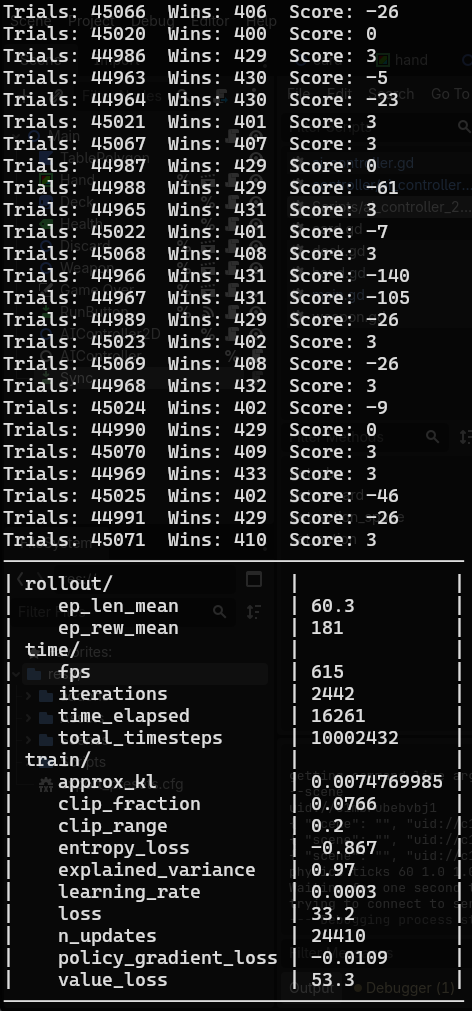
\includegraphics[width=\textwidth]{firstSuccess.png}
    \caption{First Success}
  \end{subfigure}
  \hfill
  \begin{subfigure}{0.40\textwidth}
    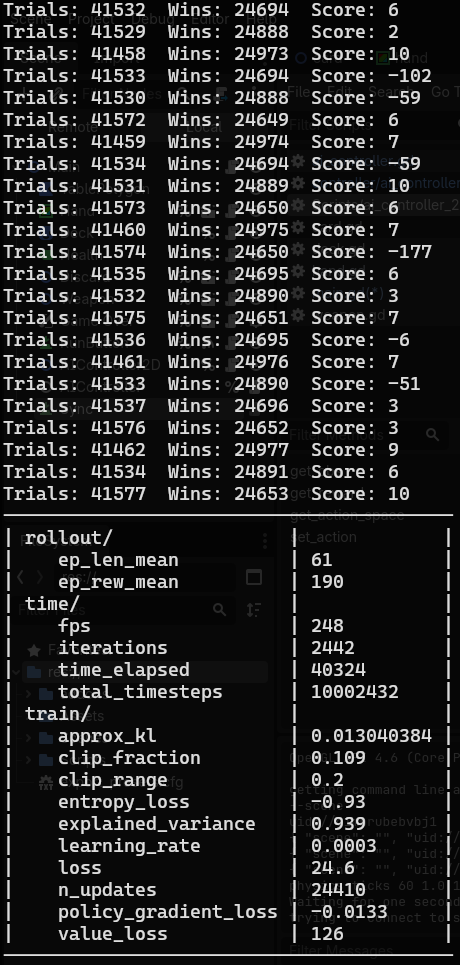
\includegraphics[width=\textwidth]{model.png}
    \caption{Same Deck Reran}
  \end{subfigure}
\end{figure}

We can see that the second time, the model got lucky and found a winning combination of choices much earlier. As I was watching it, it happened at about 8,000 trials total. It also finds a much better final score of 10, so we can run many trials, but may not find the best solution considering how many possible combinations there are.

\newpage
The second test was another success with a new deck, but I had been checking to see if the deck was beatable, and the previous two were. With the third trial, I wished to see if the model could find a solution where I couldn't, so it was given a deck I couldn't beat after a few attempts. Below are the second and third tests:

\begin{figure}[h!]
  \centering
  \begin{subfigure}{0.4\textwidth}
    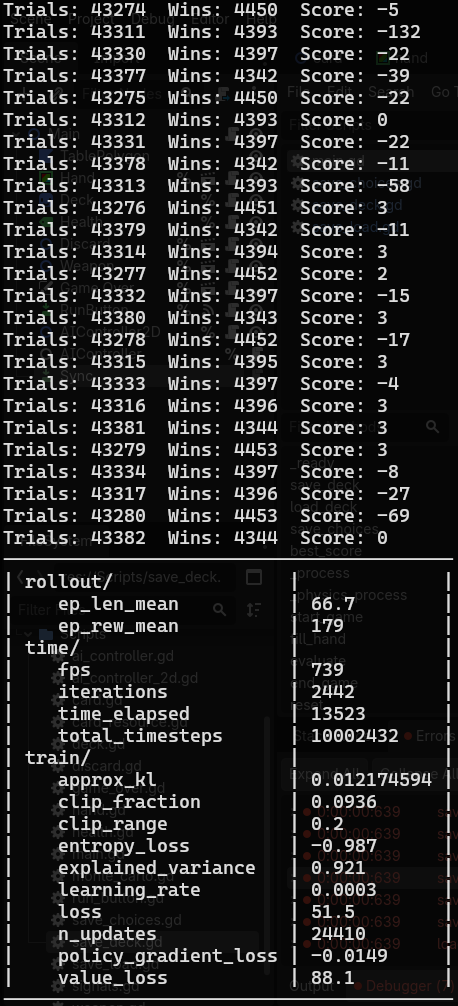
\includegraphics[width=\textwidth]{Trial2.png}
    \caption{Second Test}
  \end{subfigure}
  \hfill
  \begin{subfigure}{0.44\textwidth}
    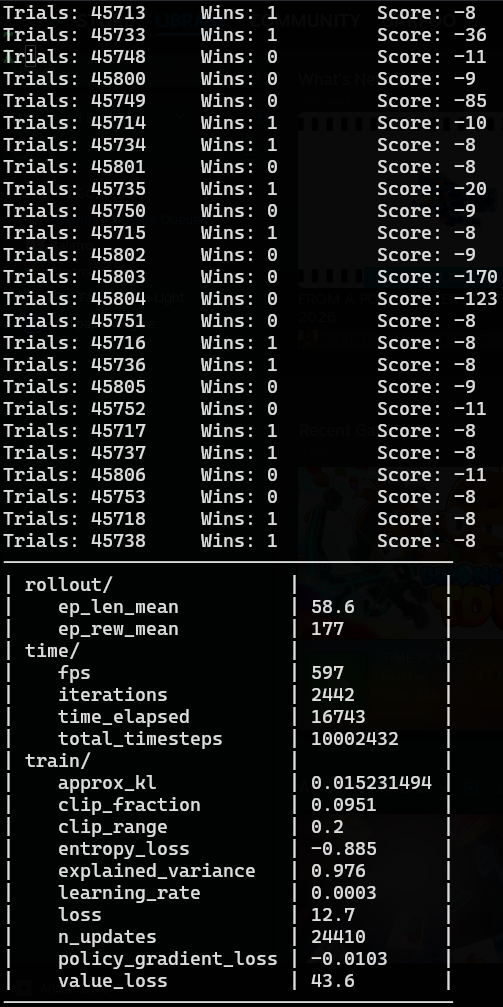
\includegraphics[width=\textwidth]{Trial3.png}
    \caption{Third Test}
  \end{subfigure}
\end{figure}

The third test was unsuccessful in finding a winning solution, but not necessarily because the deck is unbeatable. It only scored a couple of wins, but the first was around 80,000 total trials, so about halfway through. It then converges on -8, meaning that a winning solution was possible but may have had many runs involved which would have lowered the reward. To alleviate this problem of losing the best solution, I implemented a program to save the best solution once the current best score has been beaten.

A fourth test was ran with a new deck and a final max score of zero. Its choice list, along with all of the trials' models are located in the Github Repository \url{https://github.com/ColbysPrograms/ScoundrelRL}

\newpage
\section{Future Considerations}
Potential future considerations could include:
\begin{itemize}
  \item Hyperparameter Tuning. The hyperparameters were changed manually based on the model's performance, like increasing the entropy coefficient if the model wasn't exploring enough.
  \item Different Algorithms. Monte Carlo Tree Search would have been a better choice for the objective of finding a winning list of choices for an individual shuffle of the deck since it does not need to repeat the same path to ensure repeatability like PPO does.
  \item Optimizing the observation space. Currently the observation space does not include the values of each card. Doing so drastically increases the potential observation spaces from $20 \cdot 9 \cdot 13 \cdot 2 \cdot 4(4) = 74,880$ to $20 \cdot 9 \cdot 13 \cdot 2 \cdot 4(4) \cdot 4(13) = 3,893,760$, so it was not included for the time and computational constraints in this project, but simplifying this relationship would be highly valuable to finding the optimal win rate for Scoundrel.
  \item Interpreting the decisions of the model. For this experiment, it searches for the best possible path to win the game. This could be observed and interpretted to find better strategies in balancing the risk of running from a room.
  \item Using exclusively Python. Much of the information for reinforcement learning and online implementations are in Python, using Gymnasium and Pygame to create the environment and using an algorithm implementation like Stable Baselines 3's implementation of PPO.
\end{itemize}

\section{Conclusion}
This project is successful in its secondary goal of finding paths that can beat the game Scoundrel, but only with sufficient time and resources. There is plenty that could be done to clean up and make a much better model, such as using a different algorithm or simplifying the observation space, but it's very similar to the current state of reinforcement learning as a whole, with constant updates and new ideas. With more fine tuning, this model could eventually be used to solve Scoundrel in general, like the original mission statement of this project.

This project's Github Repository is hosted at\\ \url{https://github.com/ColbysPrograms/ScoundrelRL}

\section{References}
\printbibliography[heading=none]

\end{document}
